Esse capítulo apresenta o ambiente simulado em que o robô evolui e no 
qual se avalia a solução ao problema SLAM. Também são descritos o modelo 
cinemático do robô e os modelos de medida inverso e direto, utilizados pelos algoritmos de estimação para predizer poses e medidas.

\section{O ambiente}
O ambiente consiste em uma espaço de 100$m^2$ delimitado por paredes e diversos ``postes'' de formato cilíndrico de 16$cm$ de diâmetro, e está representado na Figura \ref{fig:environment}.
\begin{figure}[h]
  \begin{subfigure}{.50\textwidth}
    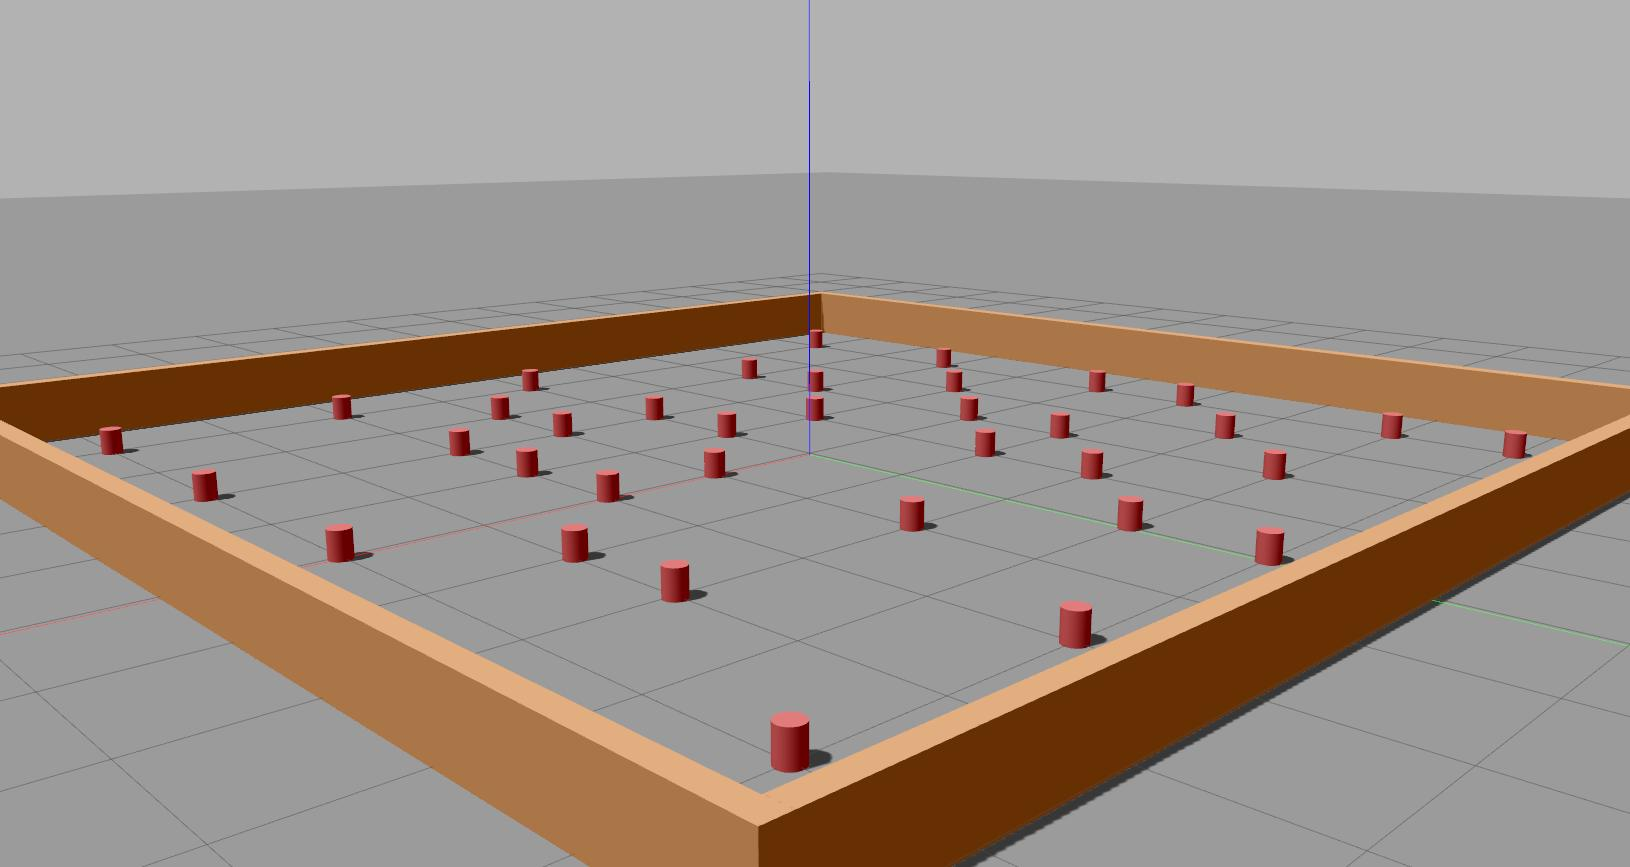
\includegraphics[width=\textwidth]{figs/environment-perspective.jpg}
    \caption{Vista perspectiva ampla}
  \end{subfigure}
  \hfill
  \begin{subfigure}{.50\textwidth}
    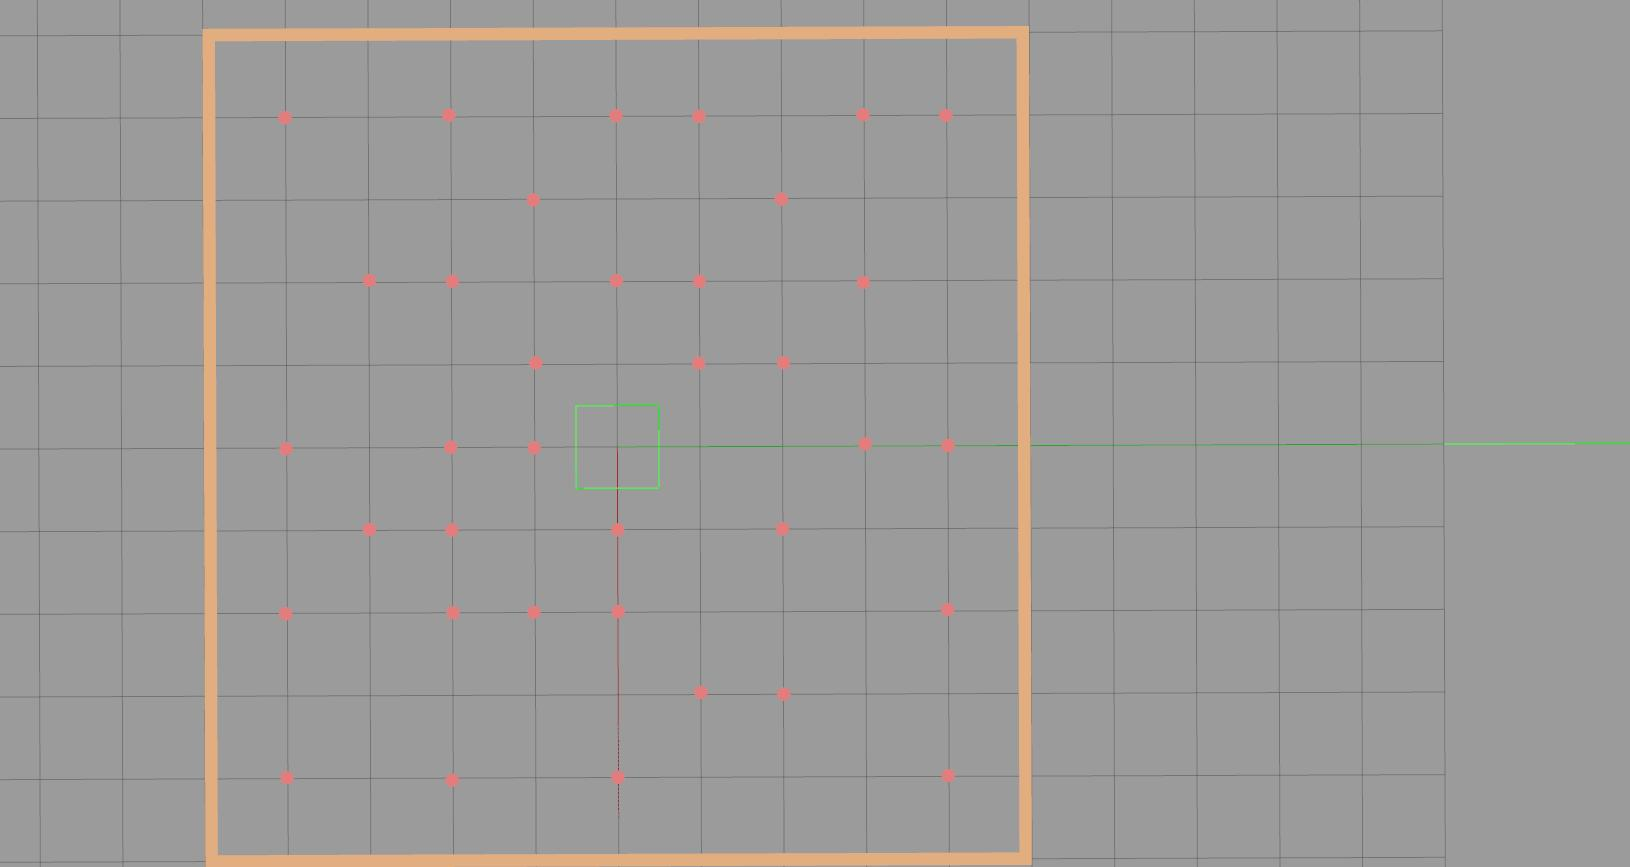
\includegraphics[width=\textwidth]{figs/environment-birds-eye-of-view.jpg}
    \caption{Vista ortográfica superior}
  \end{subfigure}
  \hfill
  \begin{subfigure}{\textwidth}
    \centering
    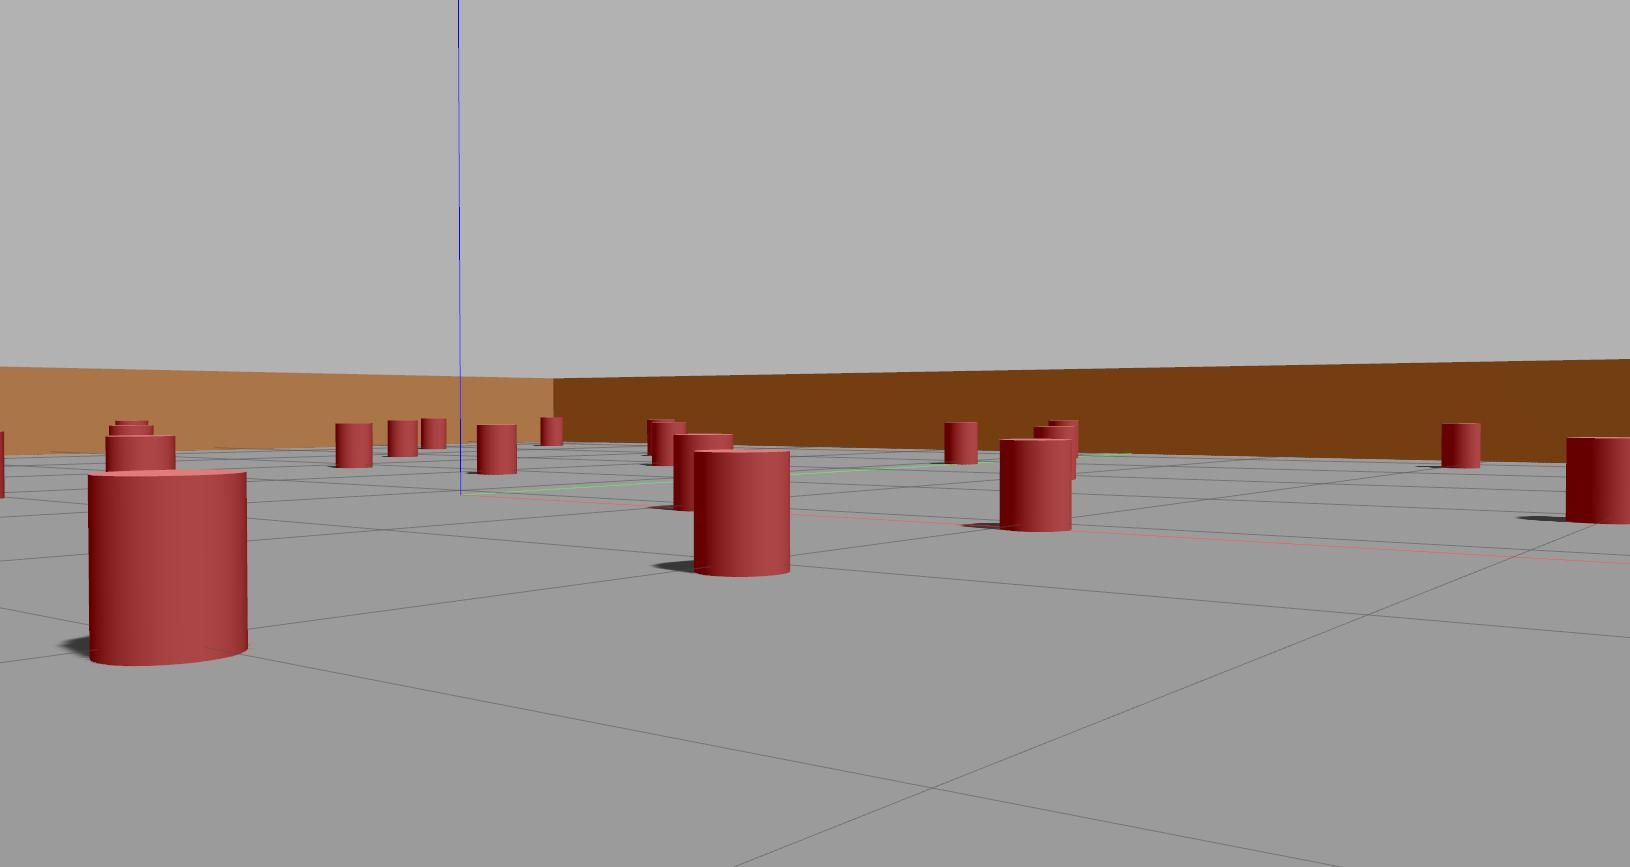
\includegraphics[width=.5\textwidth]{figs/environment-closer-perspective.jpg}
    \caption{Vista perspectiva fechada}
  \end{subfigure}
  \caption{Diferentes vistas do ambiente simulado}
  \label{fig:environment}
\end{figure}

\section{O robô}
Neste trabalho foi utilizado o modelo do robô \emph{Turtlebot 3} \cite{TurtleBot_3}, que é um robô de acionamento diferencial equipado com 
\textit{encoder} de rodas, uma IMU e um sensor laser do tipo LiDAR.
\begin{figure}[h]
  \centering
  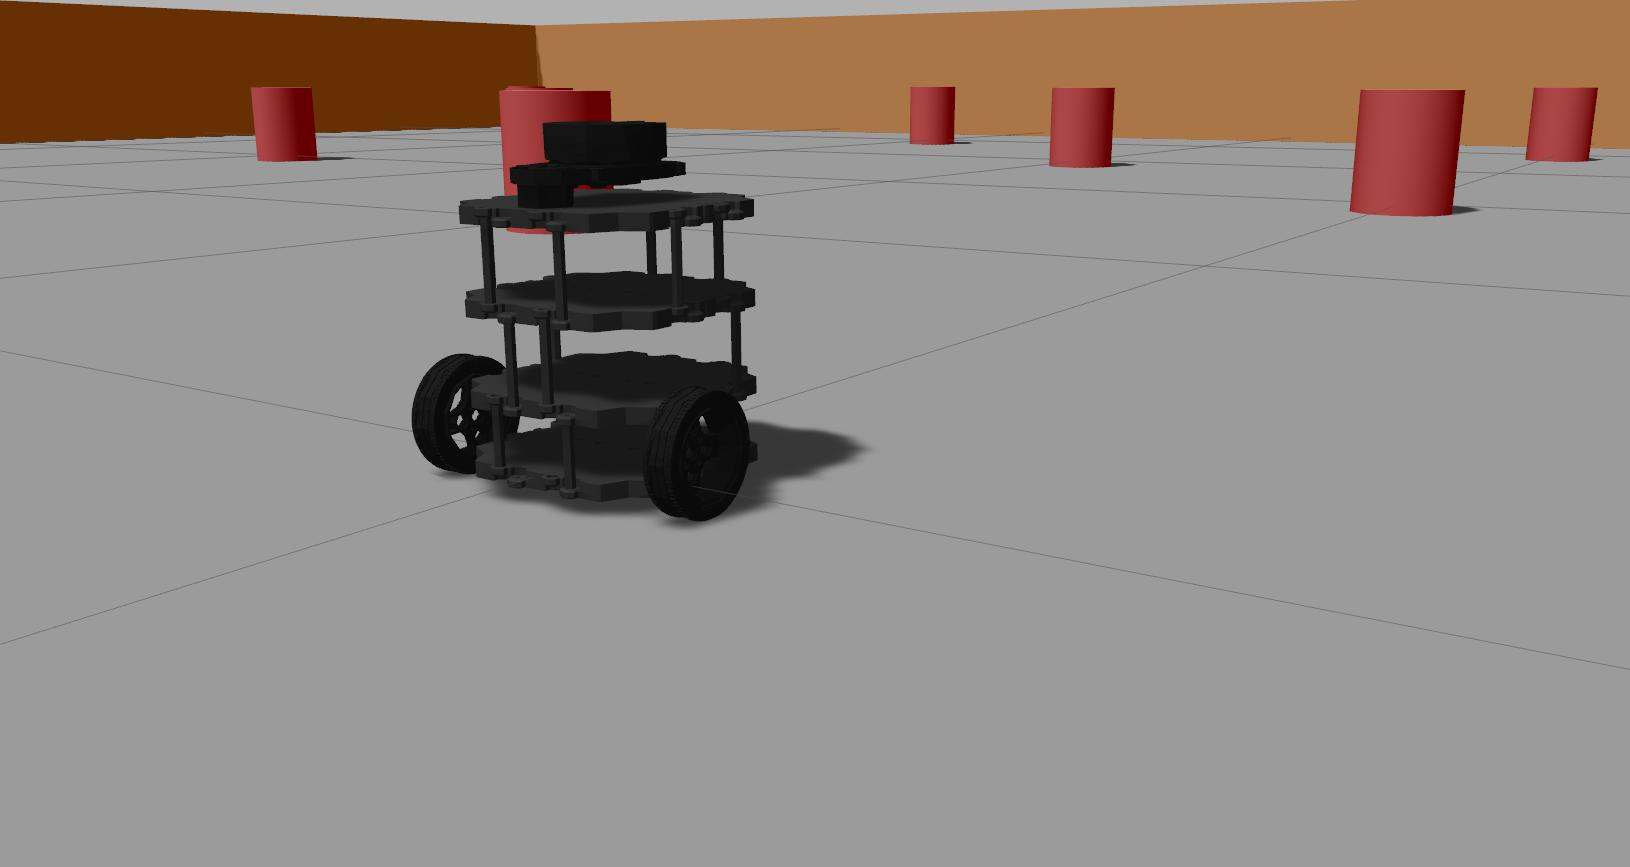
\includegraphics[width=0.7\textwidth]{figs/robot-closeup.jpg}
  \caption{Modelo do robô \textit{Turtlebot 3}. O sensor LiDAR encontra-se no topo do robô.}
  \label{fig:turtlebot-digital-twin}
\end{figure}

\subsection{Modelo do robô}
Na Figura \ref{fig:diff-drive-schematic} é representado o esquemático de um robô diferencial; as características mais importantes nesse tipo de construção 
são o raio da roda, $r$, e a distância entre os eixos das rodas, $2d$. A 
pose do robô, no instante $t$, é definida como:
\begin{equation}
  \bsubvec{x}{t} = \begin{bmatrix}
    \phi_t & x_t & y_t
  \end{bmatrix}^T
  \label{eq:robot-pose}
\end{equation}
em que $\phi$ é o ângulo do eixo $\hat{x}_r$, do sistema de coordenadas móvel 
do robô, com o eixo $\hat{x}$ do sistema de coordenadas estático $\{s\}$. E $(x, y)$ é origem do sistema de coordenadas do robô, no sistema estático.
\begin{figure}[h]
  \centering
  \includestandalone[width=0.54\textwidth]{figs/diff-drive}
  \caption{Visão superior do esquemático de um robô diferencial. O eixo z está apontando para fora 
  da folha. O sistema de coordenadas móvel do robô está posicionado no ponto médio do eixo das rodas  (cinza escuro). Na imagem, $\{s\}$ é um sistema de coordenadas estático.}
  \label{fig:diff-drive-schematic}
\end{figure}

O modelo de movimento do robô, na Equação \ref{eq:motion-model} usa apenas a informação dos \textit{encoders}. Na 
expressão abaixo, a entrada 
$\bsubvec{u}{t}$ é composta pelos deslocamentos angulares, $u_t^L$ e $u_t^R$, das rodas esquerda e direita durante o intervalo $]t-1, t]$.
\newcommand{\factor}{d\cdot\dfrac{u_t^{R} + u_t^L}{u_t^R - u_t^L}}
\begin{equation}
\begin{aligned}
  \bsubvec{x}{t} &= \mb{g}_\mathrm{r}(\bsubvec{x}{t-1}, \bsubvec{u}{t}) \\
  &= \begin{bmatrix}
      \phi_{t-1}  \\ x_{t-1} \\ y_{t-1}
    \end{bmatrix} + 
  \begin{cases}
  \renewcommand{\arraystretch}{1.8}
    \begin{bmatrix}
      \alpha_t
      \\
      \factor \parentheses{\sin(\phi_{t-1} + \alpha_t) - \sin(\phi_{t-1})} 
      \\
      \factor \parentheses{-\cos(\phi_{t-1} + \alpha_t) + \cos(\phi_{t-1})}
    \end{bmatrix}, \text{Se } u_t^L \neq u_t^R \\ 
    \\
    \renewcommand{\arraystretch}{1.1}
    \begin{bmatrix}
      0
      \\
      r\cdot u_t^R \cos(\phi_{t-1}) 
      \\
      r\cdot u_t^R \sin(\phi_{t-1}) 
    \end{bmatrix}, \text{Caso contrário}
  \end{cases}
\end{aligned}
\label{eq:motion-model}
\end{equation}
\renewcommand{\arraystretch}{1}
Onde:
\begin{equation}
  \alpha_t = \dfrac{r}{2d} \parentheses{u_t^L - u_t^R}
\end{equation}
Assim como os modelos de medida na próxima Seção, o modelo de movimento do 
robô de acionamento diferencial é não linear. Portanto, é necessário calcular 
sua matriz jacobiana em torno de um ponto $\overline{\bvec{x}}_{t-1}$ para linearização do modelo em técnicas como EKF e SEIF-SLAM, apresentadas 
mais adiante. O jacobiano do modelo \robotModel{} está na Equação 
\ref{eq:motion-model-jacobian}.
\begin{equation}
  \bsubvec{G}{R} = \bvec{I}_3 + \begin{cases}
    \renewcommand{\arraystretch}{1.8}
    \begin{bmatrix}
      0 & 0 & 0 \\
      \factor \parentheses{\cos(\overline{\phi}_{t-1} + \overline{\alpha}_{t-1}) - \cos(\overline{\phi}_{t-1})} & 0 & 0 \\
      \factor \parentheses{\sin(\overline{\phi}_{t-1} + \overline{\alpha}_{t-1}) - \sin(\overline{\phi}_{t-1})} & 0 & 0  
    \end{bmatrix}, \text{Se } u_t^L \neq u_t^R \\
    \\
    \renewcommand{\arraystretch}{1}
    \begin{bmatrix}
      0 & 0 & 0 \\
      -r\cdot u_t^R \sin(\overline{\phi}_{t-1}) & 0 & 0 \\
      r\cdot u_t^R \cos(\overline{\phi}_{t-1}) & 0 & 0  
    \end{bmatrix}, \text{Caso contrário}
  \end{cases}
  \label{eq:motion-model-jacobian}
\end{equation}

\section{Medidas e o modelo de medida Distância-Azimute}
\label{sec:slam-measurement}
A medida gerada pelo sensor LiDAR, embarcado no TurtleBot, consiste em uma nuvem de pontos planar. Essa nuvem de pontos é processada e dela são extraídas estimativas dos centros dos cilindros presentes no ambiente. Esses 
centros são as medidas utilizadas pelo algoritmo de SLAM, eles são descritos 
em termos de coordenadas polares $(r, \theta)$ no sistema de coordenadas do sensor.

\subsection{Modelo de medida Distância-Azimute}
O modelo de medida calcula a medida que espera-se ser lida pelo sensor, quando o sistema está no estado $\bsubvec{x}{t}$. Na Figura \ref{fig:range-bearing-measurement-schematic}, é representado um sistema composto por um robô e três \textit{landmarks} i, j e k. Logo o vetor de estados, $\bvec{x}$, é formado pela pose do robô, e pelas posições das landmarks no mapa:
\begin{equation}
  \bvec{x} = \begin{bmatrix}
    \phi & x & y & m_x^i & m_y^i & m_x^j & m_y^j & m_x^k & m_y^k
  \end{bmatrix}^T
\end{equation}
O modelo de medida para a j-ésima \textit{landmark} é dado por
\renewcommand{\arraystretch}{1.5}
\begin{equation}
  \mb{h}^j(\bvec{x}) = \begin{bmatrix}
    r^j \\ \theta^j
  \end{bmatrix} = \begin{bmatrix}
    \sqrt{(m_x^j - x_l)^2 + (m_y^j - y_l)^2} \\
    \arctan\left(\dfrac{m_y^j - y_l}{m_x^j - x_l}\right) - \phi
  \end{bmatrix}
  \label{eq:range-bearing-measurement-model}
\end{equation}
\renewcommand{\arraystretch}{1}
sendo
\begin{equation}
  \begin{cases}
    x_l = x + d \cos \phi\\
    y_l = y + d \sin \phi
  \end{cases}
\end{equation}

\begin{figure}[h]
  \centering
  \includestandalone[width=\textwidth]{figs/range-bearing}
  \caption{Esquemático do modelo de medida Distância-Azimute. O sistema de coordenadas do robô é representado em magenta, e o sistema de coordenadas do sensor em azul. A medida $(r^j, \theta^j)$ se refere à i-ésima \textit{landmark} no mapa.}
  \label{fig:range-bearing-measurement-schematic}
\end{figure}

Como o modelo de medida em \ref{eq:range-bearing-measurement-model} é não linear, é necessário linearizá-lo para soluções como EKF-SLAM e seus derivados, como SEIF-SLAM. Sua matriz jacobiana, $\bvec{H}$ para a j-ésima \textit{landmark}, descrita na Equação \ref{eq:measurement-model-jacobian-full}, 
ela é composta pelos jacobianos $\bsubvec{H}{\mathrm{r}}$, calculado com relação à pose do robô, e pelo jacobiano $\bsubvec{H}{M}$, calculado com relação à 
posição da \textit{landmark} no vetor de estado.
\renewcommand{\arraystretch}{2}
\begin{equation}
  \bsubvec{H}{\mathrm{r}}^j = \begin{bmatrix}
    \dfrac{d}{r^j}\parentheses{\delta_x \sin\phi - \delta_y \cos\phi} &  \dfrac{-\delta_x}{r^j} & \dfrac{-\delta_y}{r^j}\\
    -\parentheses{\dfrac{d}{\brac{r^j}^2}\parentheses{\delta_y \sin\phi + \delta_x \cos\phi} + 1} & \dfrac{\delta_y}{\brac{r^j}^2} & \dfrac{-\delta_x}{\brac{r^j}^2}
    \end{bmatrix}
  \label{eq:measurement-model-jacobian-robot-part}
\end{equation}
\renewcommand{\arraystretch}{2}
\begin{equation}
  \bsubvec{H}{\mathrm{m}}^j = \begin{bmatrix}
      \dfrac{\delta_x}{r^j} & \dfrac{\delta_y}{r^j} \\
      \dfrac{-\delta_y}{\brac{r^j}^2} & \dfrac{\delta_x}{\brac{r^j}^2}
    \end{bmatrix}
  \label{eq:measurement-model-jacobian-map-part}
\end{equation}
\renewcommand{\arraystretch}{1}
\begin{equation}
  \bvec{H}^j(\bvec{x}) = \begin{bmatrix}
    \bsubvec{H}{\mathrm{r}}^j & \bsubvec{0}{2\times 2} & \cdots & \bsubvec{H}{\mathrm{m}}^j & \cdots & \bsubvec{0}{2\times 2}
  \end{bmatrix} 
  \label{eq:measurement-model-jacobian-full}
\end{equation}

\subsection{Modelo de medida inverso Distância-Azimute}
\label{sec:inverse-measurement-model}
O modelo de medida descrito na Seção anterior é também conhecido como modelo de medida direto, pois descreve a medida que espera-se ler quando o sistema está em um dado estado. Mas também há o modelo de medida inverso, que informa sobre o estado a partir de uma medida. Esse modelo é útil durante o descobrimento de novas \textit{landmarks}, pois ele dá meios para que suas posições sejam  incorporadas ao vetor de estados. Na Figura \ref{fig:range-bearing-inverse-model-schematic} está representado o momento no qual o robô descobre a p-ésima \textit{landmark} do ambiente.
\begin{figure}[h]
  \includestandalone[width=\textwidth]{figs/range-bearing-inverse}
  \caption{Esquemático do modelo de medida Distância-Azimute. O sistema de coordenadas do robô é representado em magenta, e o sistema de coordenadas do sensor em azul. Os círculos representam \textit{landmarks}, as conhecidas pelo robô (portanto presentes no vetor de estados), em cinza, e recém descobertas, em laranja. A p-ésima \textit{landmark} acaba de ser encontrada pelo robô.}
  \label{fig:range-bearing-inverse-model-schematic}
\end{figure}

O modelo de medida inverso \invMeasurementModel{} é descrito na Equação \ref{eq:inverse-measurement-model}. Como pode ser observado, assim como o 
modelo de medida ``direto'', o modelo de medida inverso é não linear e requer linearização para o EKF-SLAM e seus 
algoritmos derivados. Sua matriz jacobiana, $\bvec{F}$, na Equação \ref{eq:inverse-measurement-model-jacobian-full} é composta pelos jacobianos 
parciais em relação ao vetor de estados, $\bvec{F}_X$, e à medida da nova 
landmark encontrada, $\bvec{F}_Y$, mostrados nas Equações \ref{eq:inverse-measurement-model-jacobian-state-part} e \ref{eq:inverse-measurement-model-jacobian-measurement-part}, respectivamente.

\begin{equation}
  \mb{f}(\bvec{x}, \bvec{y}^{p}) = 
    \begin{bmatrix}
        m_x^p \\
        m_y^p \\
    \end{bmatrix} =
    \begin{bmatrix}
        x_l + r^p \cos(\phi + \theta^p)\\
        y_l + r^p \sin(\phi + \theta^p) 
    \end{bmatrix}
    \label{eq:inverse-measurement-model}
\end{equation}

\begin{equation}
  \bvec{F}_X = 
    \begin{bmatrix}
      \begin{bmatrix}
          -d \sin{\phi} - r^p \sin(\phi + \theta^p)  & 1 & 0\\
          d\cos{\phi} + r^p\cos(\phi + \theta^p) & 0 & 1
      \end{bmatrix} & \nullmat{2}{n-3} \end{bmatrix}
  \label{eq:inverse-measurement-model-jacobian-state-part}
\end{equation}

\begin{equation}
  \bvec{F}_Y = \begin{bmatrix}
       \cos(\phi + \theta^p) & -r^p\sin(\phi + \theta^p)\\
       \sin(\phi + \theta^p) & r^p\cos(\phi + \theta^p)
    \end{bmatrix}   
  \label{eq:inverse-measurement-model-jacobian-measurement-part}
\end{equation}

\begin{equation}
  \bvec{F} = \begin{bmatrix}
    \bvec{F}_X & \bvec{F}_Y
  \end{bmatrix}
  \label{eq:inverse-measurement-model-jacobian-full}
\end{equation}

% \section{Simulação}

% \section{Visualização}
